\chapter{Vizualizační knihovna}\label{sec:Implementation2}

Tato knihovna slouží pro vizualizaci průchodu regulárním výrazem.
Pro získání informací o vyhledávání, slouží již zmíněná knihovna, která byla popsána v předchozí kapitole \ref{sec:Implementation1}.
Hlavním cílem této části aplikace je, na implementovat uživatelsky přívětivé a intuitivní rozhraní.
To umožňuje zadávat regulární výrazy, text ve kterém lze pomocí zadaného výrazu vyhledávat a následnou vizualizaci ve formě debuggeru.

%TODO

\section{Návrh}

Vstupem knihovny HTML soubor \textit{main.html}.
Ten vkládá skript \textit{index.ts}, jehož hlavním účelem je inicializovat vše potřebné pro chod aplikace.
Hlavní třídou, která se stará o obsluhu vizualizace je RegexVisualizer. 
Jejím úkolem je obsluhovat ostatní komponenty a přímo komunikuje s třídou \textit{Regexer} a tím získává data pro vizualizaci.
Pro interakci uživatele slouží dva textové editory, ty jsou ve formě dvou tříd \textit{RegexEditor} a \textit{StringMatchEditor}.
Obsluhují HTML elementy pro zadávání textu, jejich základní funkcionalita je děděna ze třídy \textit{TextEditor}.
Pro samotnou vizualizaci ve formě ladícího nástroje, existuje třída \textit{RegexDebugger}.
Má za úkol, obsluhovat okno aplikace, kde se samotný debugger nachází.
Obsahuje i vlastní posuvník (\textit{Slider}), který dokáže vyvolávat události, s informací o aktuální hodnotě posuvníku.
Také má například možnost automatického přehrávání a změnu rychlosti.

%TODO

%TODO: change loc
\subsection*{Komunikace s třídou regexer}

%TODO

\section{Implementace textových editorů}

Ve vizualizaci se nachází dva textové editory, pro zadávání regulárního výrazu a druhý pro zadávání řetězce, ve kterém proběhne vyhledávání na základě zadaného výrazu.
Jejich funkcionalita je obalena ve dvou třídách, každá sloužící pro jiný textový editor a obě dědí ze třídy \textit{TextEditor}.
Tento vztah lze vidět na obrázku \ref{fig:TextEditor}.

\begin{figure}[!h]
	\centering
	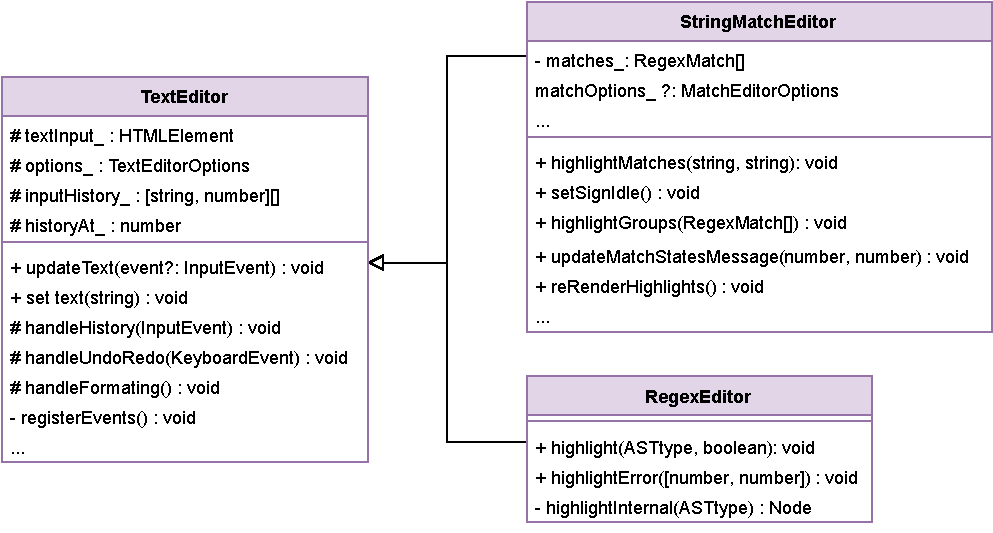
\includegraphics[width=0.8\textwidth]{Figures/TextEditor.pdf}
	\caption{Třídní diagram textových editorů}
	\label{fig:TextEditor}
\end{figure} 

\subsection*{Základní řešení}

Pro řešení textových editorů, jsem se rozhodl pro vlastní implementaci, pro větší flexibilitu a řešení konkrétních problému, týkajících se práce s regulárními výrazy.
Textový editor umožňuje rozšířené možnosti práce s textem, oproti HTML elementům, jako jsou input nebo textarea.
Tyto možnosti jsou například vlastní formátování, nebo správa historie. 
K realizaci samotných vstupů, jsem použil základní obalující HTML blok span.
Na zvoleném bloku tolik nezáleží, ale je potřeba, aby měl atribut \textit{contenteditable}, s nastavenou hodnotou na true.
Tento atribut povoluje psaní přímo do daného bloku. 
Oproti elementu jako je input, lze zde vkládat HTML kód a tím upravovat formátování textu.
To je vhodné pro regulární výrazy, jelikož sami o sobě nejsou moc přehledné.

\textit{TextEditor} slouží jako vzorová třída, pro realizaci textových editorů.
Drží si referenci na HTML element, který obsluhuje, pod názvem \textit{textInput\_}. 
Pro interaktivitu s tímto elementem, je potřeba zaregistrovat různé události.
Mezi ně patří např. psaní, mazání, undo a redo. 
Události jsou registrovány při vytvoření instance třídy, pomocí soukromé metody \textit{registerEvents}.
Pokud je zavolána, chráněná metoda \textit{handleFormating}, tak dojde ke změně podoby textu na formátovanou.
Jedná se o grafické zobrazení bílých znaků, jako je nový řádek nebo tabulátor.

%TODO
% TODO: mby add element helper

\subsection*{Zvýraznění syntaxe}

Součástí třídy \textit{RegexEditor}, je metoda sloužící pro zvýrazňování syntaxe regulárních výrazů. 
Pro zvýraznění slouží získaná AST struktura po dokončeném parsování.
Algoritmus řešení tohoto problému, funguje na principu rekurzivního zanoření, ve stromové struktuře.
Každý symbol, který má být zvýrazněný, je obalený v HTML bloku, s třídou identifikující o jaký symbol se jedná.
U jednotlivých vzorů, záleží na pořadí zpracování symbolů a rekurzivního zanoření.
Například skupina, se zpracovává tak, že první se zvýrazní otevírací závorka "(".
Poté se algoritmus rekurzivně zanoří, nebo-li zpracuje potomky (vnitřní část) skupiny a nakonec zvýrazní ukončující závorku ")".
Výsledkem vznikne HTML struktura, která popisuje symboly a vzory regulárních výrazů.
Tyto symboly jsou pak zvýrazněny, pomocí různých barev, definovaných v CSS.

\subsection*{Historie}
Práci s historii jsem musel na implementovat vlastní, jelikož původní nefungovala správně.
Důvodem bylo časté přepisování textu, z již zmíněného formátování.
Aby historie fungovala, musel jsem vytvořit pole, které obsahuje jak původní řetězec tak pozici kurzoru v něm.
Pokud byla vyvolána operace vrácení se zpět v historii (undo), překopíruje se uložený řetězec do textového pole a kurzor se nastaví na správnou pozici.
K odstranění záznamu z historie nedochází, jelikož může být vyvolána \textit{redo} operace, nebo-li odvolání operace \textit{undo}.
Pokud dojde k uložení nového stavu textového pole, tak všechny stavy za ukazatelem se smažou a přidá se zde nový.
V nastavení editoru, jsem přidal možnost zvolit si maximální počet záznamů v historii.
Pokud ale není nastavená, automaticky se omezí na 100 záznamů.

\subsection*{Pozice textového kurzoru}
Práce s textovým kurzorem je další značná část textových editorů.
Pokud uživatel píše do textového pole, často nastává ke změně textu na pozadí samotnou aplikací.
Například při zvýraznění, dochází ke změně textové formy na HTML strukturu.
Při změně vždy dojde k resetování pozice kurzoru v textu.
To ale pro uživatele není příjemná vlastnost, kterou jsem tedy musel vyřešit.

Před přepsáním textového pole, je uložená pozice kurzoru.
Po vložení textu, je nutné vrátit se na uloženou pozici. 
Nejedná se ale o jednoduchou úlohu, jelikož pokud se v textu nachází HTML elementy, musí být brány v potaz.
Použil jsem základ algoritmu ze stránky \textit{stackoverflow}\footnote{https://stackoverflow.com/questions/69956977}, který dokáže jak zjistit aktuální pozici kurzoru, tak z pozice umístit kurzor na správné místo.
Ten jsem upravil pro potřeby mého projektu a dále rozšířil.
Například jsem přidal možnost vytvoření nového kurzoru, který není přímo vložený do dokumentu, což se může hodit pokud je potřeba získat souřadnice písmena.

\section{Vizualizace průchodu}

Vizualizace ve formě debuggeru je obsluhována třídou \textit{RegexDebugger}.
Okno pro vizualizaci se otevře po kliknutí na tlačítko, které je předáno třídě součástí konstruktoru.
Debugger obsahuje identická pole jako textová pole pro interakci s uživatelem, avšak již nelze jejich text editovat.
Dále disponuje posuvníkem, který slouží pro procházení průběhu vyhledávání. 

\subsection*{Posuvník}

Posuvník jsem zvolil, jako jednoduchou a intuitivní možnost procházení historie.
Jeho implementace je ve vlastní třídě a jeho součástí je nastavení, pro příjemnější manipulaci výsledného posuvníku.
Pomocí nastavení, lze vypínat/zapínat některé funkcionality, nebo měnit samotný vzhled, jako je barva či velikost.
Tato realizace je vlastní, z důvodu lehčí integrace do aplikace.

Při vytváření instance této třídy, musí být předán HTML element nebo id elementu, do kterého se posuvník vykreslí.
Nastavení je dobrovolné, pokud není předáno zvolí se základní.
Posuvník může mít tlačítka pro ovládání, těmi jsou automatické přehrávání, vpřed, zpět, na konec a na začátek.
Pro automatické přehrávání, může být součástí pole, pro editaci rychlosti, pokud je povolené v nastavení.

Posuvník může nabývat pouze celočíselných hodnot, v omezeném rozmezí od \textit{min} do \textit{max}.
Pokud se změní jeho hodnota, je vyvolána vlastní událost, která tuto hodnotu obsahuje.
Ta může být odchycena, např. jinou třídou.

\subsection*{Zvýraznění pozice a backtrackingu}

Pro vizualizaci slouží zvýraznění pozice, jak v regulárním výrazu, tak v hledaném řetězci.
Tento koncept jsem převzal z inspirativní stránky \textit{regex101.com}.
Pozice je zvýrazněná tak, že je v pozadí pozice barevný blok, který je vykreslený do HTML plátna (canvas).
Řešení tohoto problému, jsem několikrát změnil, jelikož se původní řešení ukázalo neúčinným v některých případech.

Jako první řešení, jsem zvolil získání šířky písmene, výšky řádku a velikost mezery mezi písmeny.
Poté jsem procházel celí řetězec a pokud byl znak součástí pozice pro zvýraznění, tak jsem rozšířil šířku zvýrazněného bloku o šířku písmene a velikost mezery.
Jesli byl nalezen znak nového řádku, nebo délka zvýrazněného bloku přetekla velikost řádku, tak jsem vytvořil nový blok pro nový řádek.
Problém tohoto řešení byl takový, že když došlo k nekontrolovanému zalomení řádku tzn. pokud byl zalomen řádek dříve, než konec tohoto řádku.
To mohlo nastat, například pokud se zalomilo slovo.
Ve výsledku docházelo k zvýraznění prázdného místa a také k jeho nesprávnému konci.

Druhé řešení, které jsem zkusil na implementovat, bylo pomocí využití textového kurzoru.
Princip byl již jiný, jelikož nebylo třeba znát velikost písmene a mezery.
Kurzor jsem nejprve umístil, na začáteční pozici zvýraznění. 
V cyklu, jsem postupně posouval kurzorem až na konec zvýraznění.
Během tohoto procesu jsem si ukládal souřadnice, kde se nachází.
Tento způsob již zamezil problému při zalamování řádku, ale byl poměrně neefektivní a dokázal zpomalovat uživatelskou interaktivitu.

Poslední zpusob implementace, dokáže vyřešit i zmíněný problém se zpomalením.
Vychází z předchozího popisu, jelikož také využívá kurzor.
Rozdílem je, že kurzor je vložen jako rozsah od začátku až po konec zvýraznění.
Není tedy třeba procházet, písmeno po písmenu.
Kvůli toho jsem upravil kód, pro získání a nastavení pozice kurzoru, tak aby umožňoval také výběr.
Tato implementace se ukázala jako nejlepší, z důvodu výkonu a funkcionality.

Pokud je pozice délky nula, nebo-li \textit{min} je stejný jako \textit{max}, tak je stále zobrazena. 
Její šířka, je pak velikost mezery mezi dvěma písmeny. 
Dále jsem musel zohlednit, jestli text má scrollbar. 
Pokud ano, tak samotné zvýraznění musí být v plátně posunuto, o výšku aktuálního scrollu.

Backtracking je vyhodnocený stejnou funkcí, jako pro zvýraznění pozice.
Jediná věc, která se liší, je forma zobrazení. 
Ta je ve tvaru šipky, signalizující odkud a kam se přesouvá v regulárním výrazu.
Výška šipky není stejná, jako výška řádku, ale je zkrácená konkrétně na 2 pixely.

\subsection*{Zobrazení skupin}

Skupiny jsou podobně zobrazeny, jako pozice vyhledání, nebo-li zvýraznění části textu.
Jelikož skupiny mohou být vnořené, je třeba předem určit pořadí, ve kterém se budou zakreslovat.
Kdyby nebyly řazeny, tak by se mohlo stát, že vnější skupina přepíše vnitřní.
Pro samotné zobrazení, je potřeba měnit barvu každé skupiny, nebo zvolit jiný způsob rozlišení, aby je bylo možné rozeznat.
Zvolil jsem první způsob, kdy podle indexu skupiny je zvolená její barva.

\section{Uživatelské rozhraní}

Základní zobrazení, je ve tmavém režimu, které lze vidět na obrázku \ref{fig:GeneralUI}.
Rozhraní je koncipováno pouze na jednu stránku a obsahuje poměrně jednoduché ovládání.
Základem rozhraní jsou dvě textová pole, kde první slouží pro zadávání regulárních výrazů a druhé pro hledaný řetězec.
Oba vstupy aplikace automaticky vyhodnocuje, nicméně vstup pro hledaný řetězec, čeká nějakou dobu, než uživatel dopíše, aby častá aktualizace nezpomalovala aplikaci.

Po dokončeném zpracování, se v pravé spodní části aplikace nachází informace, které jsou vidět na obrázku \ref{fig:GeneralUI}.
Zobrazuje se zde, kolik úspěšných vyhledání se povedlo a v kolika krocích.
Také vedle zmíněných informací, je umístěna ikona signalizující informaci o průběhu zpracování.
Ikona může být zobrazena čtyřmi různými způsoby.
První je ukázán na obrázku a jedná se o celkový úspěch vyhledání.
Další 3 ikony značí neúspěch, načítání resp. zpracovávání a poslední čekání na správně zadaný regulární výraz.

V levé spodní části aplikace je tlačítko pro otevření debuggeru, po jeho otevření se zobrazí okno, které je ukázáno na obrázku \ref{fig:DebuggerUI}.
Na vrchu okna se nachází, posuvník který slouží pro průchod stavů.
S ním souvisí tři pole, které jsou pod posuvníkem.
Aktuální stav, nebo-li hodnota posuvníku, se nachází v levém poli.
Uprostřed je ovládání pomocí pěti tlačítek: začátek, zpět, automatické přehrávání, dopředu a konec.
Poslední políčkem souvisejícím s posuvníkem, je pro manipulaci rychlosti automatického přehrávání.
Rychlost je pak vyjádřena, jako $1/n$ stavů za sekundu, kde $n$ je nastavená rychlost, v případě obrázku \ref{fig:DebuggerUI} je $n = 5$.

Dále se v debuggeru nachází dvě pole, pro vizualizaci stavů regulárního výrazu a druhé pro vizualizaci pozice v hledaném řetězci.
Stavy jsou automaticky aktualizovány, po změně hodnoty posuvníku.
V regulárním výrazu v obrázku, je zrovna vyobrazen backtracking (červená šipka zpět).
V hledaném řetězci, se zvýrazněná pozice, aktuálního stavu vyhledávání.
Jeho součástí mohou být zobrazeny skupiny, pokud nějaké již byly dokončeny.

\begin{figure}[!h]
	\centering
	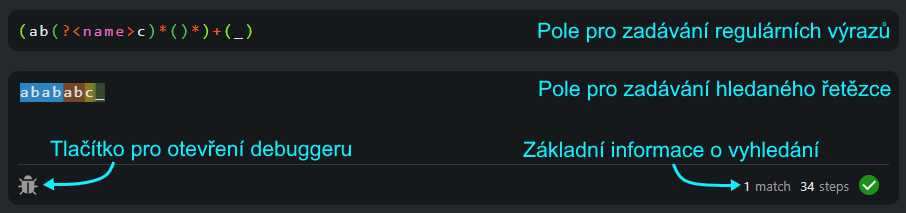
\includegraphics[width=0.85\textwidth]{Figures/appWindow.png}
	\caption{Úvodní uživatelské rozhraní}
	\label{fig:GeneralUI}
\end{figure}

\begin{figure}[!h]
	\centering
	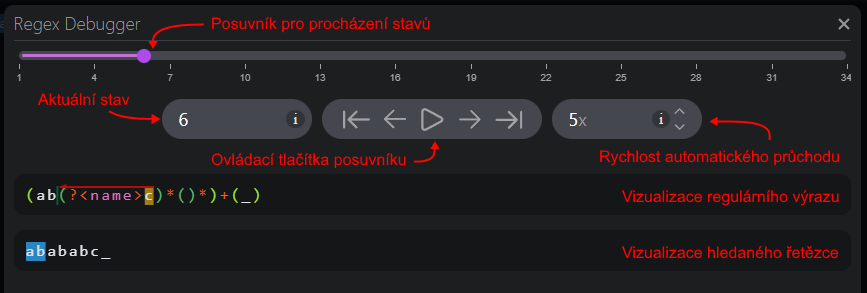
\includegraphics[width=0.85\textwidth]{Figures/appDebugger.png}
	\caption{Uživatelské rozhraní debuggeru}
	\label{fig:DebuggerUI}
\end{figure}

VSCode api zpřístupňuje využití css stylů, které má uživatel přímo nastavené ve svém prostředí.
Pokud je tedy webová stránka součástí VSCode prostředí, tak přejímám styly, které má uživatel přímo nastavené.
Součástí toho jsou, fonty, barvy, tmavý nebo světlý režim atd.
Jestliže má uživatel nastavený světlý režim, tak se stránka automaticky přizpůsobí.

\endinput